\documentclass[../main.tex]{subfiles}
\graphicspath{{\subfix{..}}}
\begin{document}
\chapter{Graph representation of JUNO for IBD reconstruction}
\epigraph{``The Answer to the Great Question of Life, the Universe and Everything is Forty-two''}{Douglas Adams, The Hitchhiker’s Guide to the Galaxy}
\label{sec:jgnn}
%\begin{itemize}
%  \item Introduce the concpet of reconstruction using Small + Large
%  \item Re state the context
%\end{itemize}

We previously showed, in chapter \ref{sec:jcnn}, that neural networks are relevant as reconstruction tools in JUNO. Even if they show worse performance, the combination to classical estimator could still bring improvement. We discussed the use of Convolutional Neural Network (CNN) in the previous chapter and their limitation, in particular the limitation of the image representation for the experiment.

In this chapter we propose to use a Graph Neural Network (GNN), a Neural Network specialized to process graph as presented in section \ref{sec:ml:gnn}, to overcome those limitations.

\section{Motivation}
\label{sec:jgnn:motiv}
%\begin{itemize}
%  \item Problem with the image representation
%  \item Explain that graph can be a solution
%\end{itemize}

As explained in chapter \ref{sec:juno} the JUNO sensors, the Large Photomultipliers (LPMT) and Small Photomultipliers (SPMT), are arranged on a spherical plane, pointing to the center of the detector. When trying to represent this plane as a 2D image, due to the inherent problem of the projection, some part of the image are distorted and part of the image do not have any physical meaning (see section  \ref{sec:jcnn:data}). A way to represent the data without inducing deformation is the Graph, an object composed of a collection of nodes and a collection edges representing the relation between the nodes.

From this graph representation, we can construct a neural network that will process the data while keeping the properties of it. For example the rotational invariance, i.e. the energy and radius of the event do change if we rotate our referential. An approach was already proposed in JUNO by Qian et al. \cite{qian_vertex_2021} where each node of the graph are like pixels, they represent geometric region of the detector and are connected with their neighbours. The LPMT informations are then aggregated on those nodes. The network then process the data using the equivalent of convolution but on graph \cite{defferrard_convolutional_2017}.

In this work we want to take a step further in the graph representation by including the SPMT and including a maximum of raw informations.

\section{Data representation}
\label{sec:jgnn:data}
%\begin{itemize}
%  \item First though
%    \begin{itemize}
%      \item All pmt are nodes
%      \item How to connect ? Fully connected ?
%      \item Fully connected not possible with our computng capacities: 40k * 40k -> $1.6\cdot10^8$ link -> around a Gb of adjacency matrix times edges features
%      \item Connected to neighbours -> Already done for graph convolution, cit yury paper
%    \end{itemize}
%  \item Second though
%    \begin{itemize}
%      \item Be smarter
%      \item All PMTs as nodes -> Fired
%      \item Have intermediate layer of node representing geometric section -> Mesh
%      \item Fired connected to mesh
%      \item Mesh fully connected
%      \item Aggregation while keeping raw informations
%      \item Add a "global node"
%    \end{itemize}
%  \item Present healpix for the segementation
%  \item Features for node/edges
%    \begin{itemize}
%      \item Classic infos: Q,t,X,Y,Z (add plots to show features)
%      \item Add high order informations
%      \item Harmonic analysis (present here ? Or in annex ?)
%      \item Other high order $\mathcal{A}$ and $\mathcal{B}$
%    \end{itemize}
%  \item Difficulty: nodes do not live in the same space (not same infos on fired, mesh, and io)
%  \item Need a custom message passing options
%\end{itemize}

In an ideal world we would want to have every PMTs represented as node in the graph, each PMT being hit is an informations but the fact that PMTs were not hit is also an important information. It's by being aware of the whole of the system that we are able to give meaning to a subpart. As a reminder, in the Central Detector (CD), JUNO will posses 17612 LPMTs and 25600 SPMTs for a total of 43212 PMTs. This amount of information in itself is still manageable by modern computer if it were to be used in a neural network but when defining the relations between the nodes, it become a bit more tricky.

Excluding self relation, an edge that would go from and to the same node, and considering the relation to be undirected, the edge from $A$ to $B$ is the same from $B$ to $A$, the amount of edge is given by $\frac{n(n-1)}{2}$ which for 43212 PMTs amount for $933'616'866$ edges. If we encode an information with double precision (64 bits) in what we call an adjacency matrix, each information we want to encode in the relation would consume 4 GB of data. When adding the overhead due to gradient computation during training, this would put us over the memory capacity of a single V100 gpu card (20 GB of memory). We could use parallel training to distribute the training over multiple GPU but we considered that the technical difficulty to deploy this solution was not worth the trouble.

The option of connecting PMTs node only to their neighbours could be tempting to reduce the number of edge, but this solution does not translate well in term of internal representation in memory. Edges of sparsely connected nodes can be stored in efficient manner in a sparse matrix but the calculation in itself would often results in the concretization of the full matrix in memory, resulting in an insufficient memory gain during training.


We finally decided of a middle ground where we define three \textit{families}:
\begin{itemize}
  \item The core of the graph will be composed of nodes representing geometric regions of the detector. We call those nodes {\color{Dandelion} mesh} nodes. Those mesh nodes are densely connected to each other. We keep their number of the order of magnitude of a thousand to keep the memory consumption low
  \item All the fired PMTs, PMTs that have been hit, will be represented as nodes. We call those node {\color{red} fired}. Fired nodes are connected to the mesh they geometrically belong.
  \item A final node which will hold global information about the detector and on which we will read the interaction vertex and energy. It's designated as the {\color{blue} I/O} node for input/output. This node will be connected to every mesh nodes.
\end{itemize}
Those nodes and their relations are illustrated in figure \ref{fig:jgnn:node_schema}. From this representation, we end up with three distinct adjacency adjacency matrix
\begin{itemize}
  \item A $N_{fired} \times N_{mesh}$ adjacency matrix, representing the relations between fired and mesh. Those relations are undirected.
  \item A $N_{mesh} \times N_{mesh}$ adjacency matrix, representing the relation between meshes. Those relation are directed.
  \item A $N_{mesh} \times 1$ adjacency between the mesh and I/O nodes. Those relations are undirected.
\end{itemize}
The adjacency matrix representing those relation is illustrated in figure \ref{fig:jgnn:adj}.

\begin{figure}
  \centering
  \begin{subfigure}[t]{0.6\linewidth}
    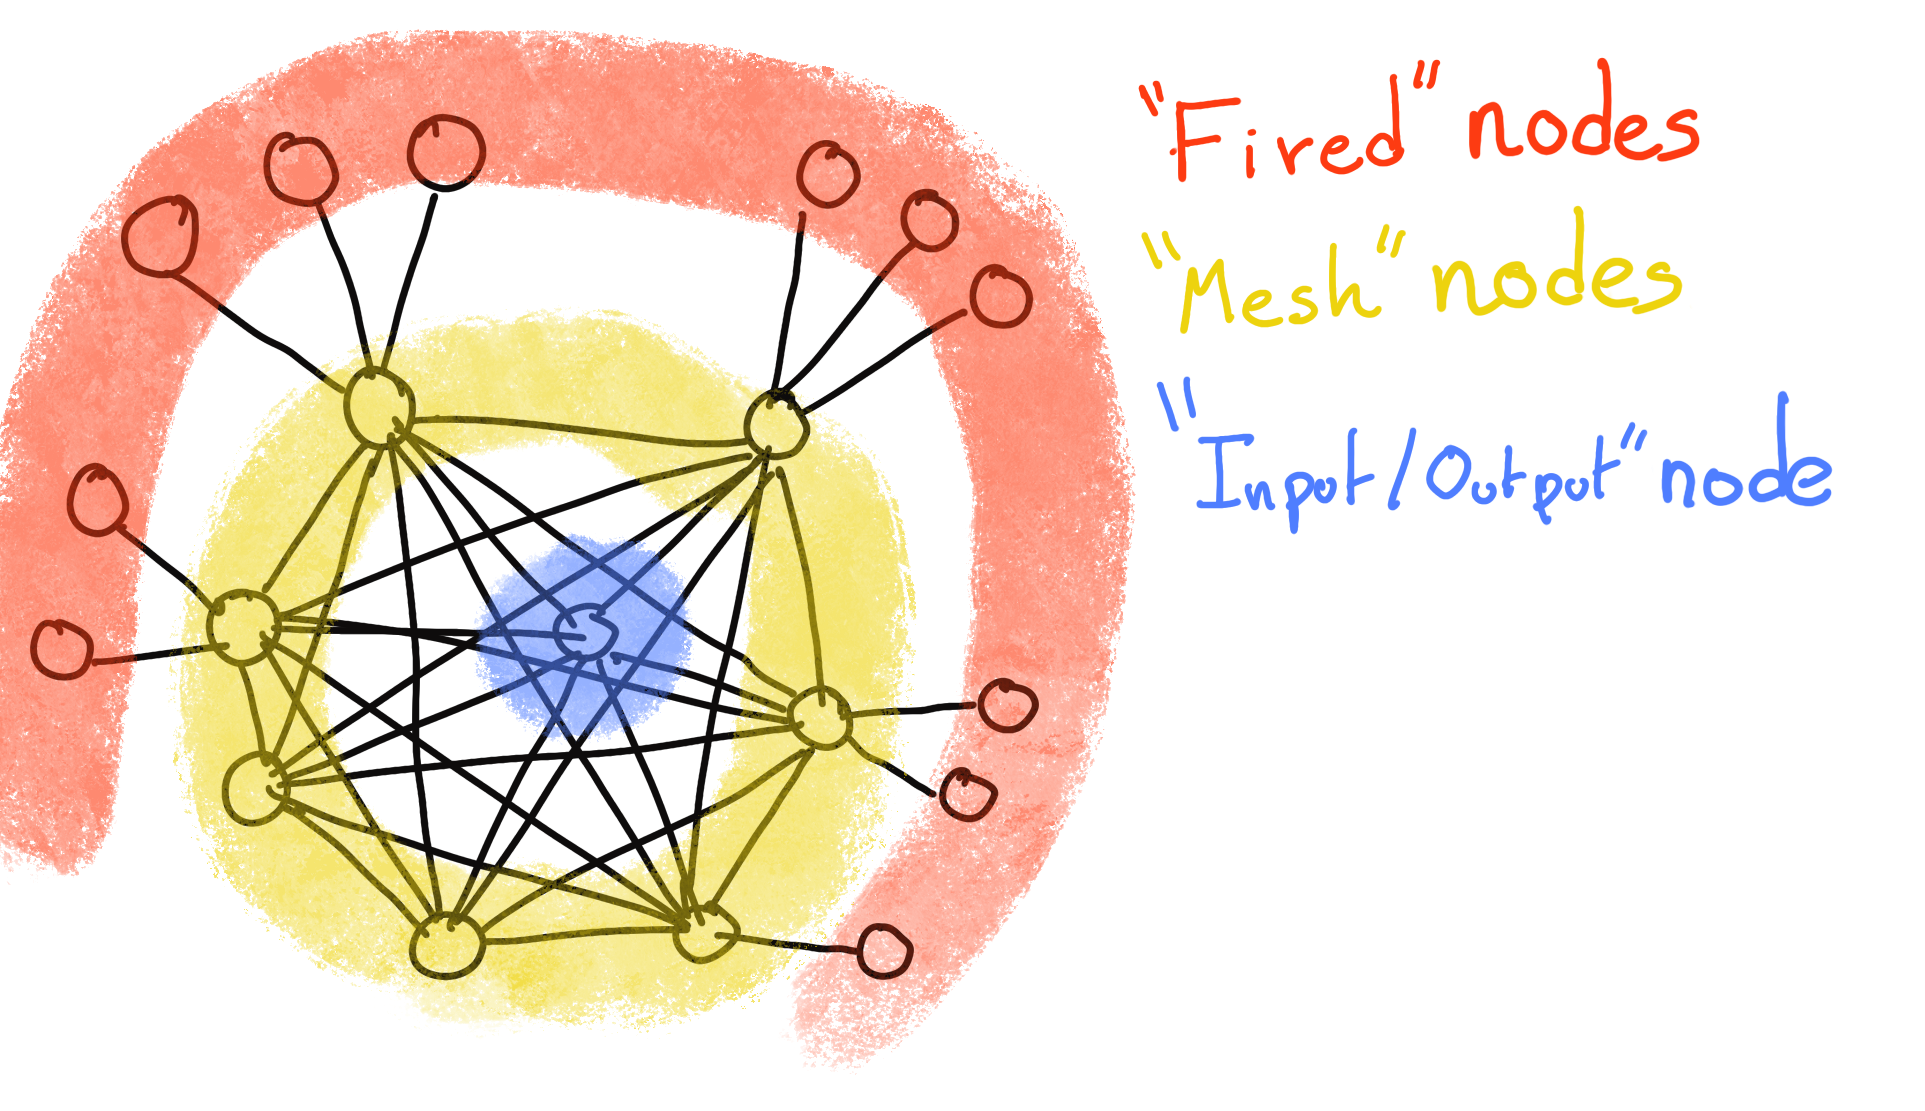
\includegraphics[width=\linewidth]{images/jgnn/nodes_schema.png}
    \caption{Illustration of the different nodes in our graphs and their relations.}
    \label{fig:jgnn:node_schema}
  \end{subfigure}
  \hfill
  \begin{subfigure}[t]{0.39\linewidth}
    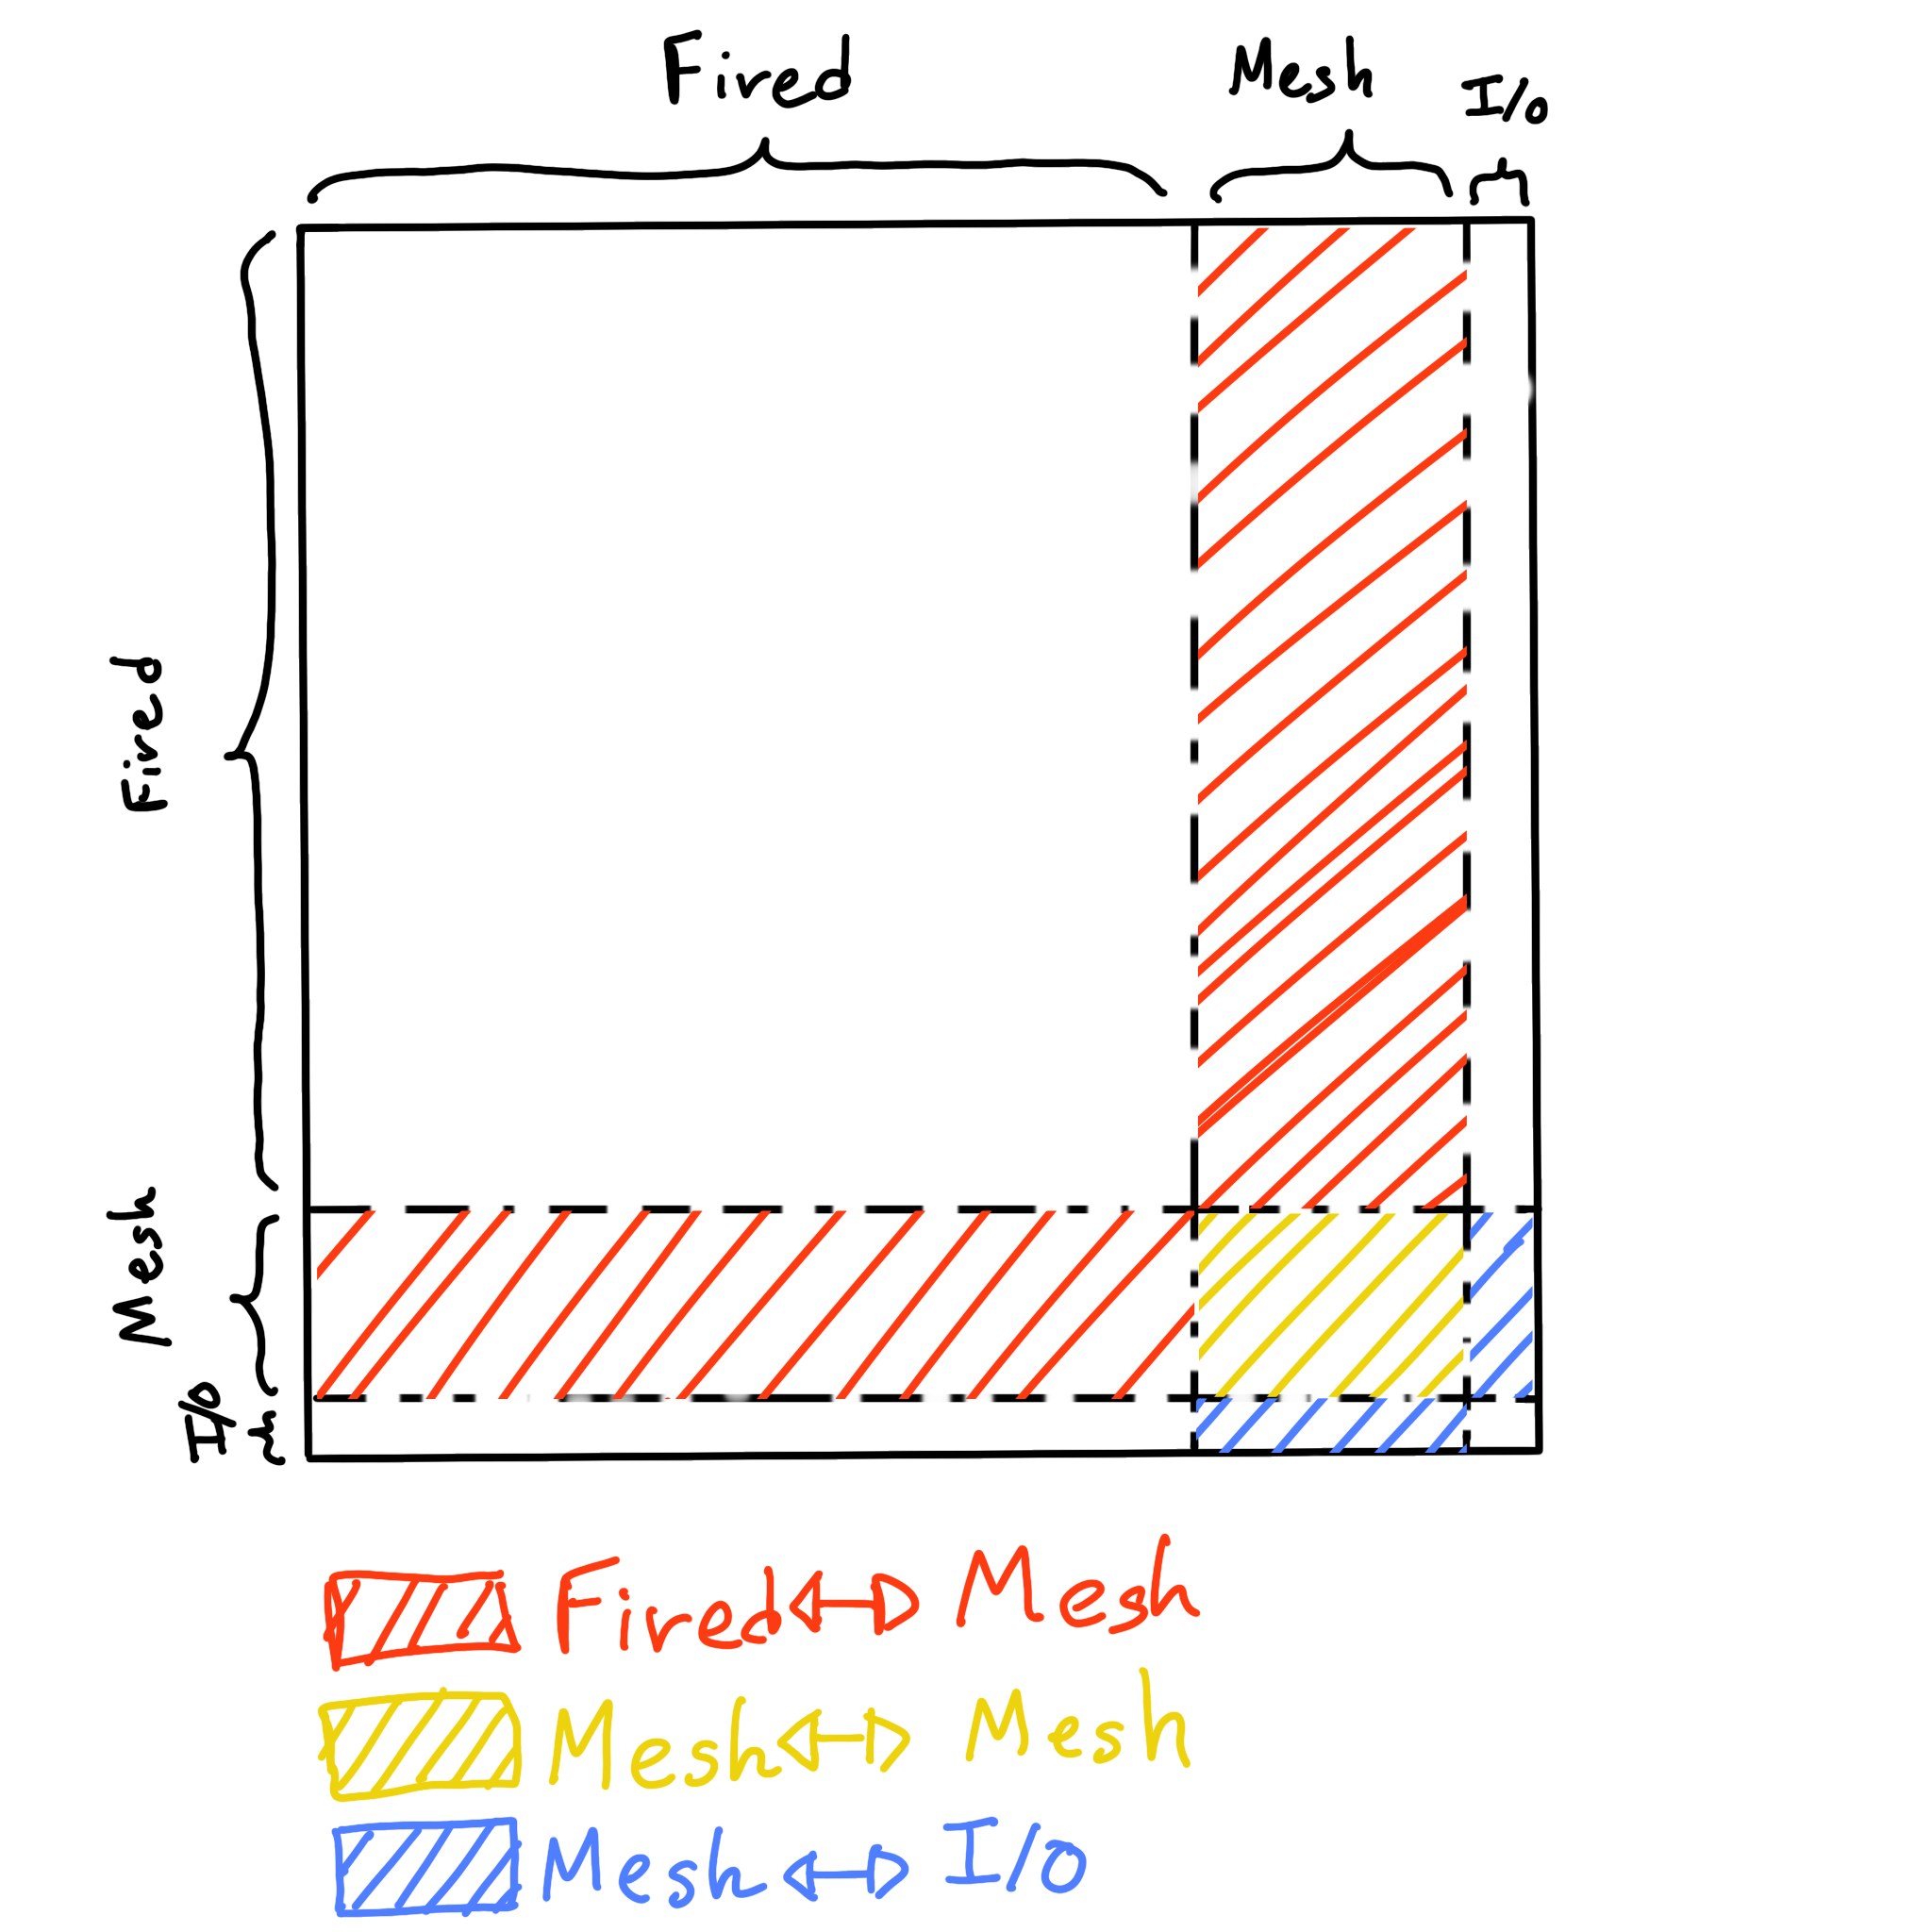
\includegraphics[width=\linewidth]{images/jgnn/adjacency_mat.png}
    \caption{Illustration of what a dense adjacency matrix would looks like and the part we a re really interested in. Because Fired $\rightarrow$ Mesh and Mesh $\rightarrow$ I/O relations are undirected, we only consider in practice the top right part of the matrix for those relations.}
    \label{fig:jgnn:adj}
  \end{subfigure}
  \caption{}
\end{figure}

The mesh segmentation is following the Healpix segmentation \cite{gorski_healpix_2005}. This segmenntation offer the advantage that almost each mesh have the same number of direct neighbours and it guarantee that each mesh represent the same extent of the detector surface. The segmentation can be infinitly subdivided to provide smaller and smaller pixels. The number of pixel follow the order $n$ with $N_{pix} = 12 \cdot 4^n$. This segmentation is illustrated in figure \ref{fig:jgnn:healpix}. To keep the number of mesh small, we use the segmentation of order 3, $N_{pix} = 12 \cdot 4^3 = 768$.

\begin{figure}
  \centering
  \begin{subfigure}[t]{0.48\linewidth}
    \centering
    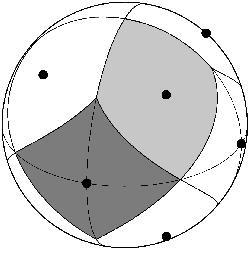
\includegraphics[width=0.5\linewidth]{images/jgnn/healpix_0.jpg}
  \end{subfigure}
  \hfill
  \begin{subfigure}[t]{0.48\linewidth}
    \centering
    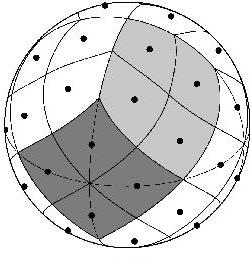
\includegraphics[width=0.5\linewidth]{images/jgnn/healpix_1.jpg}
  \end{subfigure}
  \caption{Illustration of the healpix segmentation. \textbf{On the left:} A segmentation of order 0. \textbf{On the right:} A segmentation of order 1}
  \label{fig:jgnn:healpix}
\end{figure}

We decided on having the different kind of nodes {\color{Dandelion} mesh (M)}, {\color{red} fired (F)} and {\color{blue} I/O} have different set of features. The features used in the graph are presented in figure \ref{fig:jgnn:graph_features}. Most of the features are low level informations such as the charge or time information but we include some high order features such as
\begin{enumerate}
  \item $P^h_l$: Is the normalized power of the $l$th spherical harmonic. For more details about spherical harmonics in JUNO, see annex \ref{sec:annex:jgnn:harms}.
  \item $\mathbb{A}$ and $\mathbb{B}$ are informations that represent the likeliness of the interaction vertex to be on the segment between the center of two meshes.
    \begin{align}
      \mathbb{A}_{ij} &= (\vec{j} - \vec{i})\cdot\frac{l_1}{D_{ij}} + \vec{i} \\
      \mathbb{B}_{ij} &= \frac{Q_i}{Q_2} \bigg(\frac{l_2}{l_1}\bigg)^2 \\
      l_1 &= \frac{1}{2}(D_{ij} - \Delta t \frac{c}{n}) \\
      l_2 &= \frac{1}{2}(D_{ij} + \Delta t \frac{c}{n})
    \end{align}
    where $\vec{i}$ is the position vector of the mesh $i$, $D_{ij}$ is the distance between the center of the meshes $i$ and $j$, $Q_i$ the sum of charges on the mesh $i$, $\Delta t = t_i - t_j$ where $t_i$ the earliest time on the mesh $i$ and $n$ the optical indice of the LS. $\mathbb{A}$ is the vertex to center of mesh distance ratio between $i$ and $j$ based on the time information. For $\mathbb{B}$, the charge ratio evolve with the square of the distance, so the mesh couple with the smallest $\mathbb{B}$ should be the one withe interaction vertex between its two center.
\end{enumerate}

\begin{figure}[ht]
  \centering
  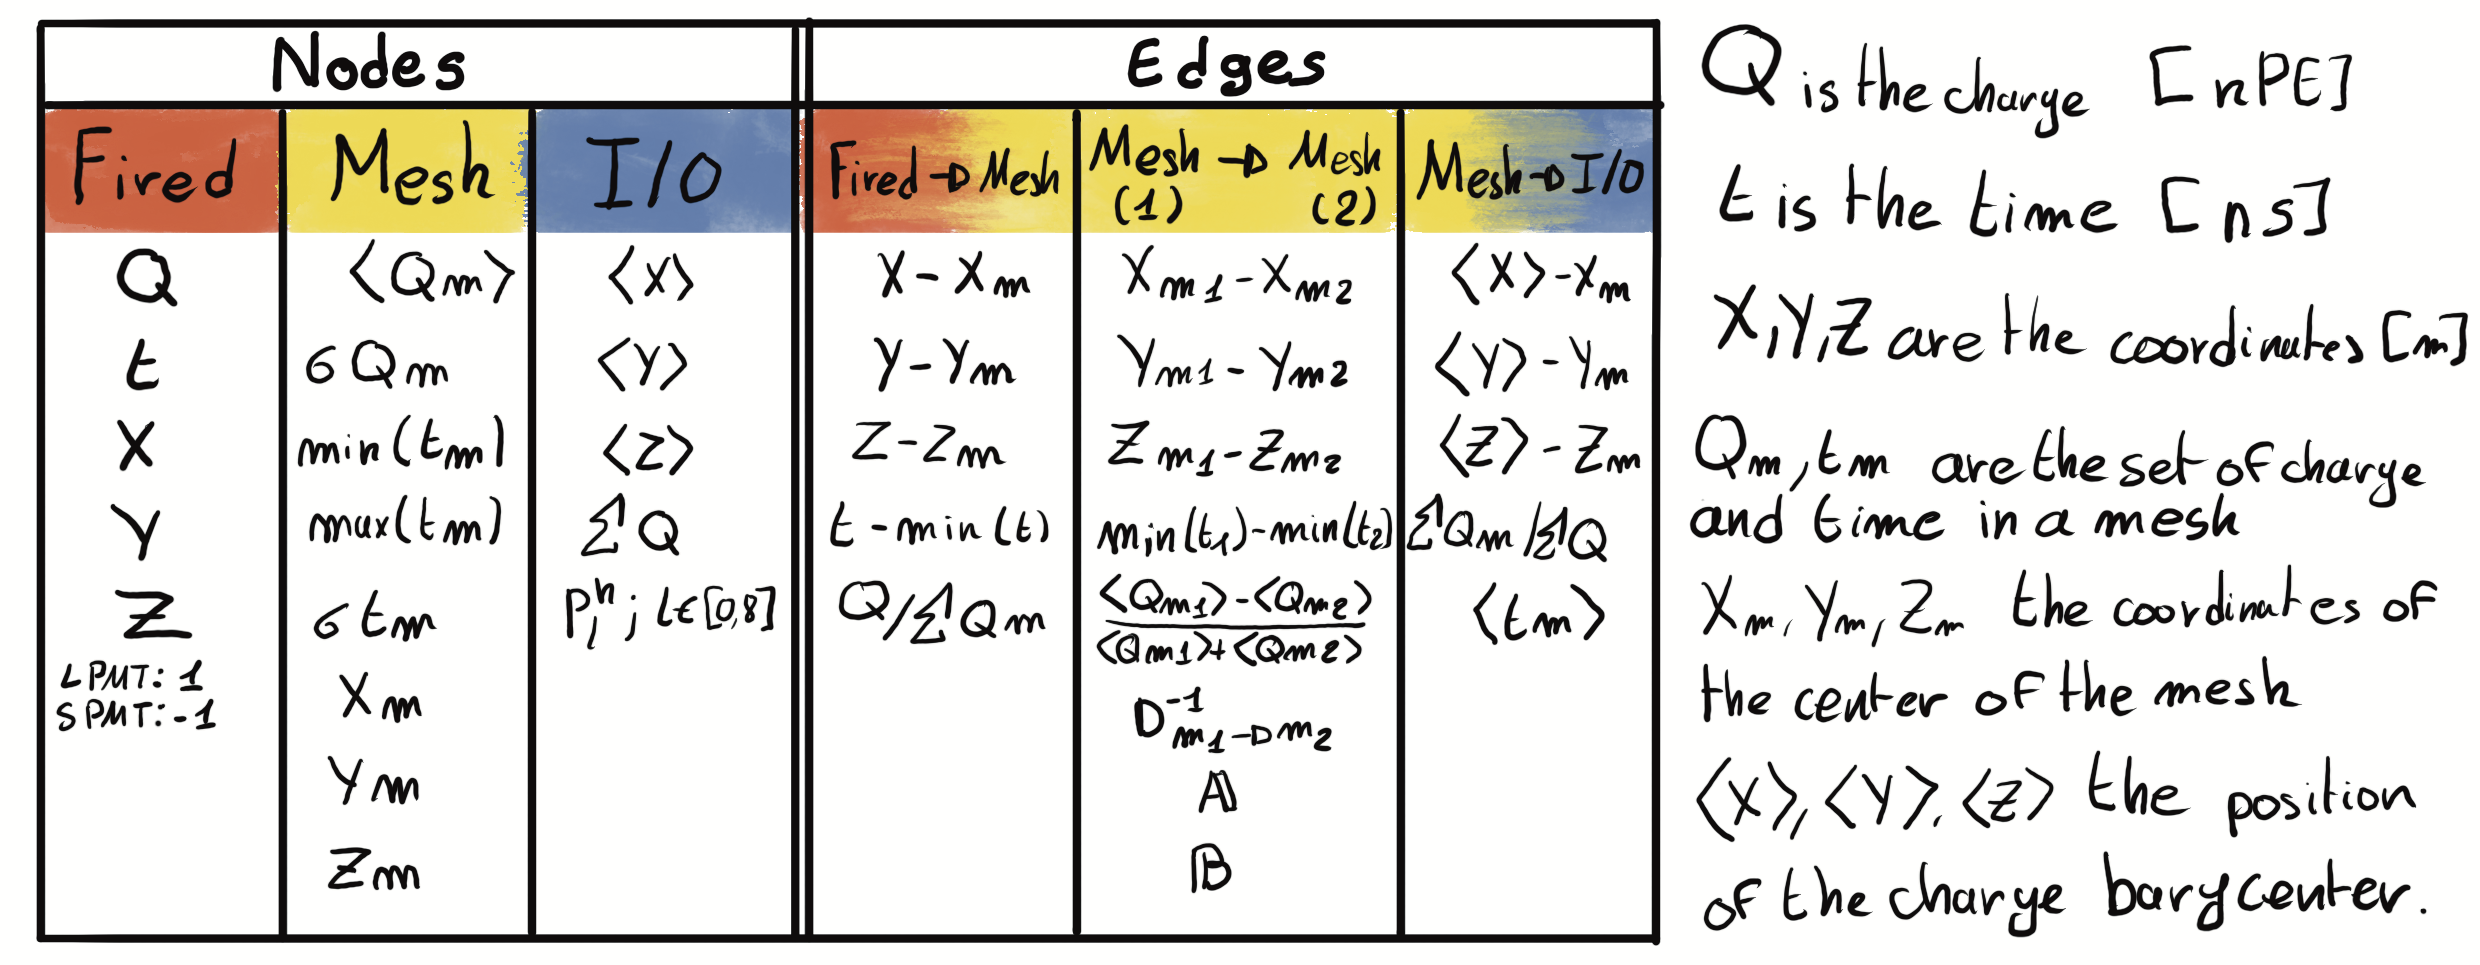
\includegraphics[height=6cm]{images/jgnn/graph_features.png}
  \caption{Features held by the nodes and edges in the graph. $D^{-1}_{m_1 \rightarrow m_2}$ is the inverse of the distane between two mesh center. The features $P^h_l$, $\mathbb{A}$ and $\mathbb{B}$ are detailed in section \ref{sec:jgnn:data}}
  \label{fig:jgnn:graph_features}
\end{figure}

Because our different nodes do not have the same number of features, they live in different spaces. Most library and public algorithms available are designed with node living in the same space in mind, we thus had to develop a custom message passing algorithm.

\section{Message passing algorithm}
%\begin{itemize}
%  \item Need one message passing algorithm per connection (f->m, m->f, m->m, n->io, io->m)
%  \item Allow to select part of the adjacency matrix (see notes)
%  \item Explain message passing layer that was developed
%  \item Reimplementation in C++ using torch framework
%  \item C++ allow also for on the fly data transformation from raw file and minutieuse memory management
%  \item Not updating the edge for the sake of technical simplicity: Commplicated to identify an edge feature from the above algorithm
%\end{itemize}
As introduced in previous section and in figure \ref{fig:jgnn:graph_features}, our graphs nodes and edges will have different number of features depending on their nature, meaning that we cannot have a single message passing function. We thus need to define a message passing function for each transition inside or outside a family. Using the notation presented in section \ref{sec:ml:gnn}
\begin{equation}
  n_i^{k+1} = \phi_u (n_i^k, \Box_j \phi_m(n_i^k, n_j^k, e^k_{ij})); ~ n_j \in \mathcal{N}'_i
\end{equation}
we need to define
\begin{align}
  \phi_{u; f\rightarrow m} ~ &\phi_{m; f\rightarrow m} \\
  \phi_{u; m\rightarrow f} ~ &\phi_{m; m\rightarrow f} \\
  \phi_{u; m\rightarrow m} ~ &\phi_{m; m\rightarrow m} \\
  \phi_{u; m\rightarrow io} ~ &\phi_{m; m\rightarrow io} \\
  \phi_{u; io\rightarrow m} ~ &\phi_{m; io\rightarrow m}
\end{align}
to update the nodes after each layers as illustrated in figure \ref{fig:jgnn:mp_ill}. We would also need update function for the edges but for the sake of technical simplicity in this work, we will limit ourself to the nodes update. A wide variety of message passing algorithm exists, with different use cases and goal behind them. To stay generalist and to match to the best the specificity of our architecture, we implement the following algorithm:
\begin{equation}
  \phi_u \coloneq I^{n'}_{i'} = I^n_i A_{i',e}^{i} W_n^{e,n'} + B^{n'}
\end{equation}
using the Einstein summation notation. $I^{n}_i$ is the tensor holding the nodes informations with $i$ the node index and $n$ the feature index. $n$ represent the features of the previous layer and $n'$ the features of this layer. $A_{n,e}^{n'}$ is the adjacency tensor, discussed in the previous section, representing the connection between the node $i'$ and the node $i$, each connecetion holding the features indexed by $e$ . The learnable weights are composed of the tensor $W_n^{e,n'}$ which represent the passage from the previous feature domain $n$, the previous layer, to the current domain $n'$, this layer knowing the relation $e$. $B^{n'}$ is a learnable bias tensor on the new features $n'$.
If a node have neighbours in different families, the different $I^{n'}_{i'}$ coming from the different $\phi_u$ are summed.
\begin{equation}
  I^{n'}_{i'} = \sum_\mathcal{N} \phi_{u,\mathcal{N}}
\end{equation}
where $\mathcal{N}$ are the neighbouring family and $\phi_{u,\mathcal{N}}$ the update function between the target node family and the neighbour $\mathcal{N}$ family.

\begin{figure}
  \centering
  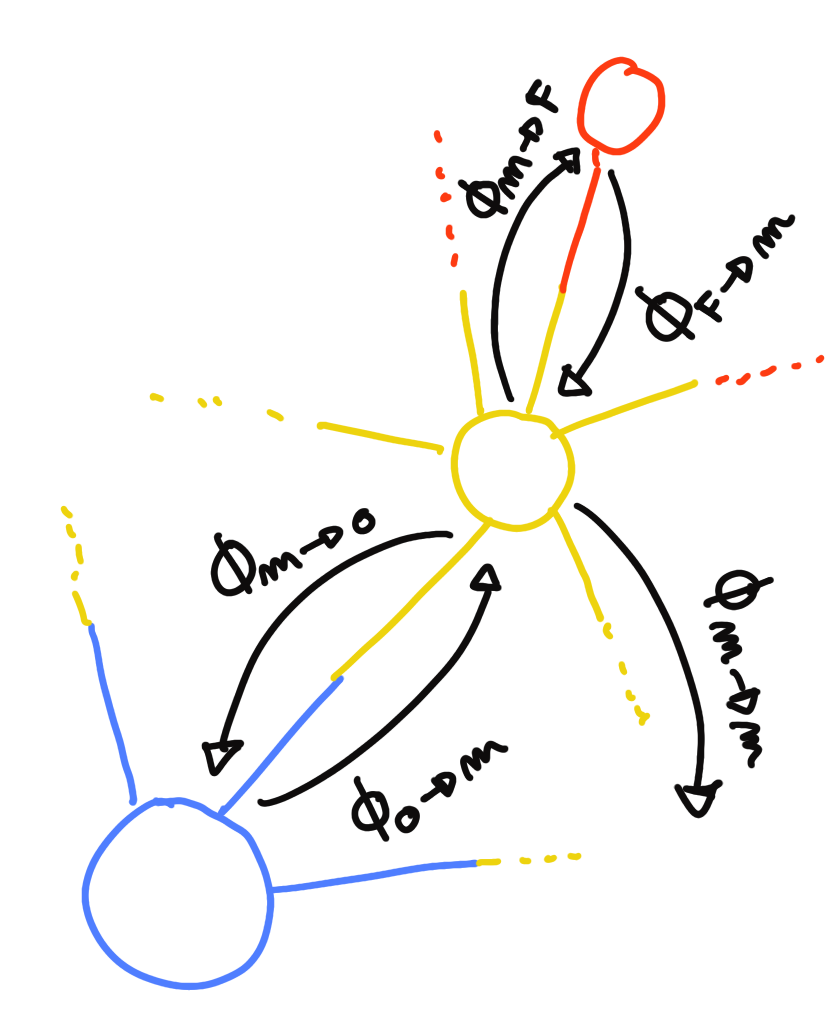
\includegraphics[height=5cm]{images/jgnn/mp_illus.png}
  \caption{Illustration of the different update function needed by our GNN}
  \label{fig:jgnn:mp_ill}
\end{figure}

We thus have a $W$ and $B$ for each of the $\phi_u$ function we defined above. The $\phi_m$ function is ``hidden'' in the Einstein sum $IAW$. Interestingly, the number on learnable weight in those layer is independent of the number of nodes in each family and depends solely on the number of features on the nodes and the edges.

This operation of message passing is the constituent of our message passing layer designed in this work \textit{JWGLayer}. To this layer, we can adjoin an activation function such as $PReLU$
\begin{equation}
  I^{n'}_{i'} = PReLU\bigg(\sum_\mathcal{N} I^n_i A_{i',e}^{i} W_n^{e,n'} + B^{n'} \bigg)
\end{equation}


\section{Data}
%\begin{itemize}
%  \item Present the data (dataset)
%  \item Maybe show an example
%\end{itemize}

For this study we will be using a 1M positrons event dataset, uniformly distributed in energy with $E_k \in [0, 9]$ MeV and uniformly distributed in the detector. Those events come from the JUNO official simulation version J23.0.1-rc8.dc1 (released the 7th January 2024). All the event are \textit{calib} level, with simulation of the physics, electronics, digitizations and triggers. 900k events will be used for the training, 50k for validation and loss monitoring and 50k for the results analysis in section \ref{sec:jgnn:results}. Each events is between 2k and 12k fired PMTS, resulting in fired nodes being the largest family in our graphs in all circumstances as illustrated in figure \ref{fig:jgnn:tot_hit_e}.

As expected, by comparing the scale between the figure \ref{fig:jgnn:lpmt_hit_e} and \ref{fig:jgnn:spmt_hit_e} we see that the LPMT system is predominant in term of informations in our data. The number of PMT hits grow with energy but do not reach 0 for low energy event due to the dark noise contribution which seems to be around 1000 hits per event for the LPMT system (left limit of figure \ref{fig:jgnn:lpmt_hit_e}) and around 15 hits per event for the SPMT system (left limit of figure \ref{fig:jgnn:spmt_hit_e}) which is consistent with the results show in section \ref{sec:jcnn:data}.

\begin{figure}[ht]
  \centering
  \begin{subfigure}[t]{0.32\linewidth}
    \centering
    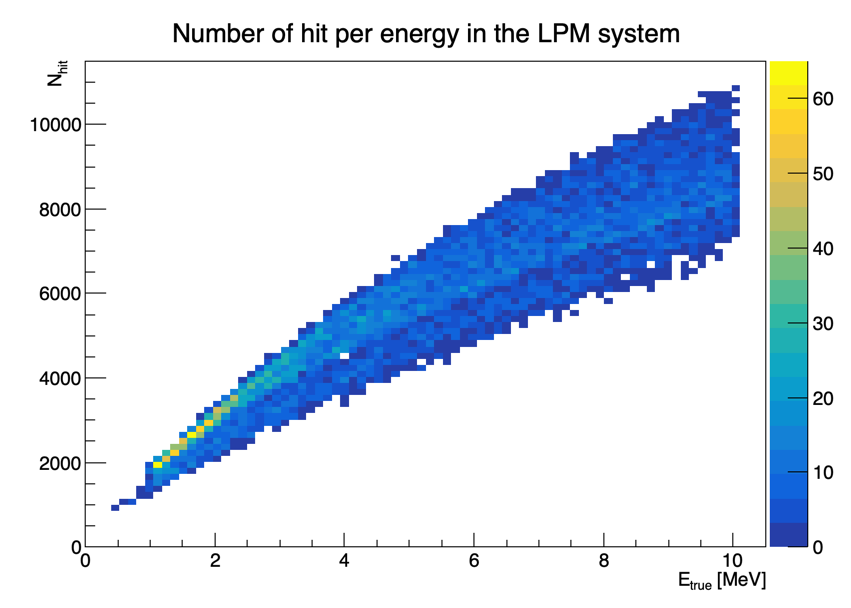
\includegraphics[width=\linewidth]{images/jgnn/lpmt_hit_e.png}
    \caption{}
    \label{fig:jgnn:lpmt_hit_e}
  \end{subfigure}
  \begin{subfigure}[t]{0.32\linewidth}
    \centering
    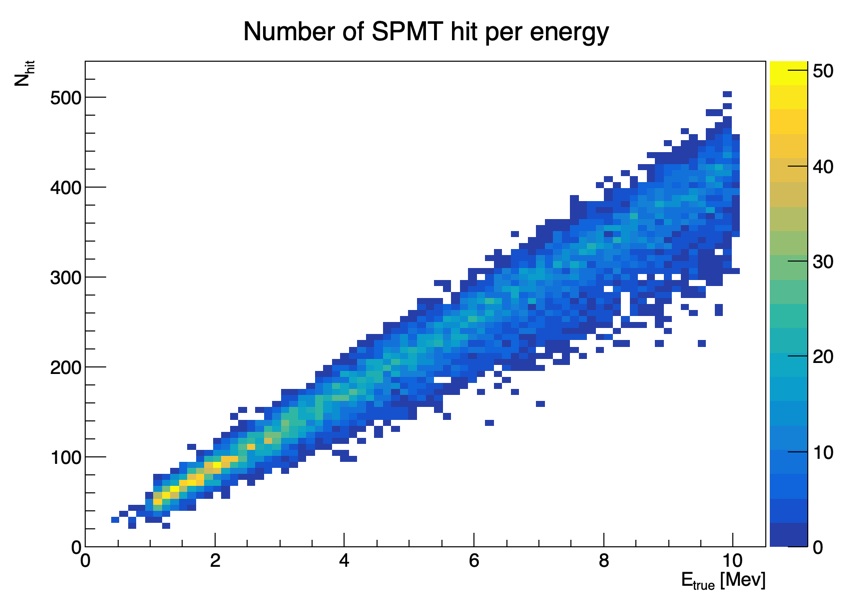
\includegraphics[width=\linewidth]{images/jgnn/spmt_hit_e.png}
    \caption{}
    \label{fig:jgnn:spmt_hit_e}
  \end{subfigure}
  \begin{subfigure}[t]{0.32\linewidth}
    \centering
    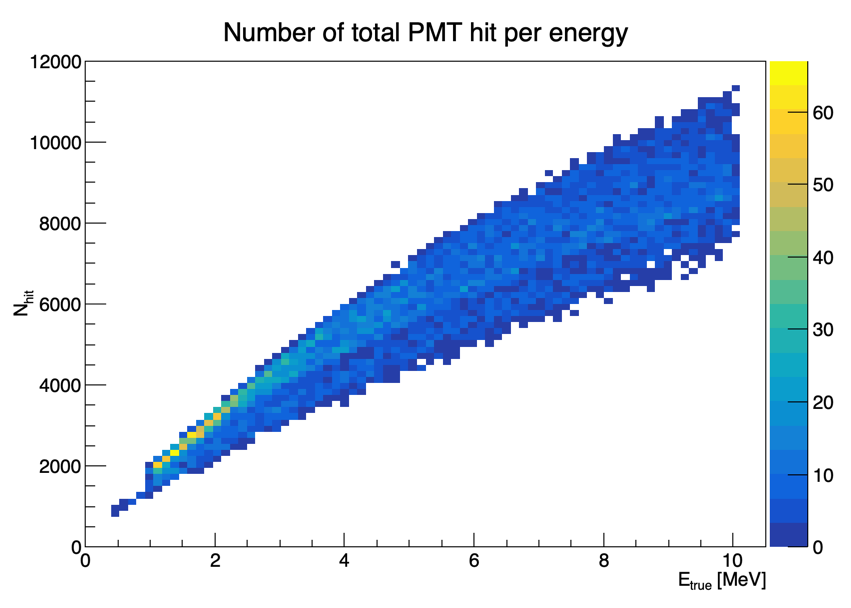
\includegraphics[width=\linewidth]{images/jgnn/tot_hit_e.png}
    \caption{}
    \label{fig:jgnn:tot_hit_e}
  \end{subfigure}
  \caption{Distribution of the number of hits depending on the energy. \textbf{On the right:} for the LPMT system. \textbf{In the middle :} for the SPMT system. \textbf{On the left: } For both system.}
\end{figure}

The structure seen in the distribution in figure \ref{fig:jgnn:lpmt_hit_e} comes from the shape of the number of hits depending on the radius as shown in figures \ref{fig:jgnn:lpmt_hit_r} and \ref{fig:jgnn:spmt_hit_r} where the number of hit decrease with radius. It is important to understand that this is not representative of the number of PE per event and the decrease in hits over the radius means that the PE are just more concentrated in a smaller number of PMTs.

\begin{figure}[ht]
  \centering
  \begin{subfigure}[t]{0.48\linewidth}
    \centering
    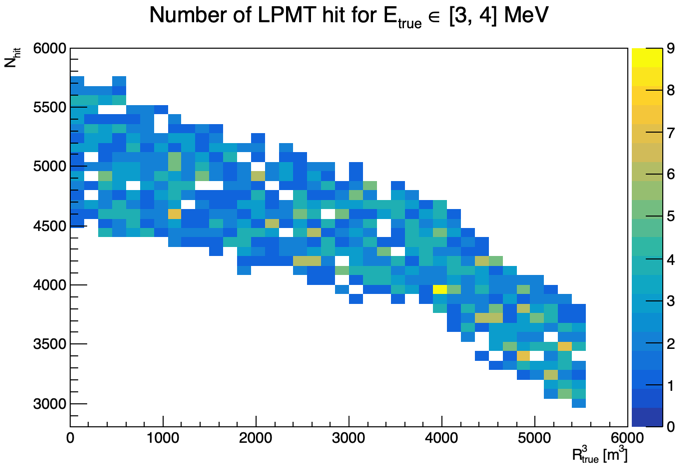
\includegraphics[width=\linewidth]{images/jgnn/lpmt_hit_r.png}
    \caption{}
    \label{fig:jgnn:lpmt_hit_r}
  \end{subfigure}
  \hfill
  \begin{subfigure}[t]{0.48\linewidth}
    \centering
    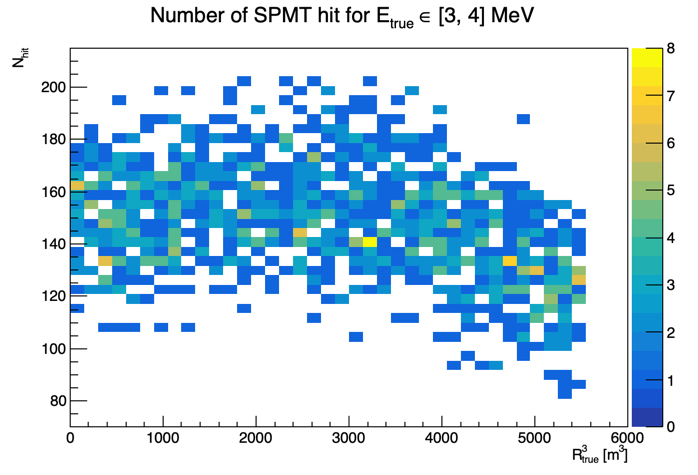
\includegraphics[width=\linewidth]{images/jgnn/spmt_hit_r.png}
    \caption{}
    \label{fig:jgnn:spmt_hit_r}
  \end{subfigure}
  \caption{Distribution of the number of hits depending on the radius. \textbf{On the right:} for the LPMT system. \textbf{On the right :} for the SPMT system. To prevent the superposition of structure of different scales we limit ourselves to the energy range $E_{true} \in [0, 9]$.}
\end{figure}



\section{Model}
%\begin{itemize}
%  \item Present number of layers etc...
%  \item Discuss hyperparameters optimisation
%  \item Random search is not viable with the accessible hardware (too time consuming) -> 90h per trainng
%  \item By hand optimization -> around 70 iterations and tests.
%\end{itemize}

In this section we'll discuss the different layer composing the final version of the model. As introduced above, each JWGLayer is defined by the number of features on the nodes and edges of the output graph, assuming it takes as input the graph from the precedent layer. For simplicity, when discussing a graph configuration, it will be presented as follow: \{ {\color{red} $N_{f}$},  {\color{Dandelion} $N_{m}$}, {\color{blue} $N_{IO}$}, $N_{f\rightarrow m}$, $N_{m \rightarrow m}$, $N_{m \rightarrow f}$ \} where
\begin{itemize}
  \item {\color{red} $N_{f}$} is the number of feature on the fired nodes.
  \item {\color{Dandelion} $N_{m}$} is the number of features on the mesh nodes.
  \item {\color{blue} $N_{IO}$} is the number of features on the I/O node.
  \item $N_{f\rightarrow m}$ is the number of features on the edges between the fired and mesh nodes.
  \item $N_{m \rightarrow m}$ is the number of features on the edges between two mesh nodes.
  \item $N_{m \rightarrow f}$ is the number of features on the edges between the mesh nodes and the I/O node.
\end{itemize}

Because we do not change the number of features on the edges, we can simplify the notation to \{{\color{red} $N_{f}$}, {\color{Dandelion} $N_{m}$}, {\color{blue} $N_{IO}$}\}. As an example, the input graph configuration, following the figure \ref{fig:jgnn:graph_features}, is \{{\color{red} 6}, {\color{Dandelion} 8}, {\color{blue} 13}, 5, 8, 5 \} or, without the edge features, \{{\color{red} 6}, {\color{Dandelion} 8}, {\color{blue} 13} \}.

The final version of the model, called JWGv7.3.0 is composed of
\begin{itemize}
  \item An JWGLayer, converting the input graph to \{ 32, 32, 32 \} with a PReLU activation function.
  \item 6 hidden JWGLayer, processing the data to \{ 32, 32, 32 \} graphs with a PReLU activation function.
  \item A flatten layer that flatten the features of the I/O and mesh nodes to a $(32 * 768 + 32) = 24608$ dimensions vector.
  \item 2 fully connected layers of 2048 neurons with a PReLU activation function.
  \item 2 fully connected layers of 512 neurons with a PReLU activation function.
  \item A final, fully connected layer of 4 neurons acting as the output of the network.
\end{itemize}

\section{Training}

The optimizer used for training is the Adam optimizer and default hyperparameters ($\beta_1= 0.9$, $\beta_2 = 0.999$ and $\epsilon = 1e-8$) with a learning rate $\lambda = $ 1e-8. The training last 200 epochs of 800 steps. We use a batch size of 8. The learning rate is constant during the first 20 epochs then exponentially decrease with a rate of 0.99. The model saved is the model with the best validation loss during the training. The validation is computed over a single batch.

\section{Optimization}

Due to the extensive training time, up to 90h per training on the more complex architectures, and the heavy memory consumption of the models that would often exceed the 20GB limit of the V100, random search was not a realistic approach to the hyper optimisation. We were able to extend the memory limit to 40GB thanks to a local A100 GPU card available at the lab.

The hyperparameters optimization was thus done ``by hand'', by looking at the results of the previous training and tinker hyperparameters that seems to play a role in the training. During this process, the model went into some heavy refactoring. At the start, the message passing algorithm was not the one presented above but each $\phi_u$ and $\phi_m$ function were FCDNN. The memory consumption and gradient vanishing caused is what made us pivot to the final message passing algorithm presented above.

Even the features on the graph went under investigation, with the addition of high level observables to the {\color{Dandelion} mesh} and {\color{blue} I/O} nodes and edge, there was too much possibility to test everything. We went with the decision to keep the raw observables in the {\color{Dandelion} mesh} and for the higher order observables we tried to take the one that would be difficult for the NN to reconstruct or at least would need multiple layer to reproduce. Basically, because the operation in the JWGLayer are linear operation, any variables dependent on order  > 1 of the input would be candidates. This is why we introduce standard deviation, $\mathbb{A}$, $\mathbb{B}$ and $P^h_l$ for example.

Substantial effort went to the data processing process before the training. Due to the volatile nature of the graph features during the optimization, the current code do not take preprocessed data and compute the observables, adjacency matrix, etc... on the fly. This data processing is carried out on the CPU, using a worker pool to allow for multiprocessing the data. The raw data are coming from root file produced by the collaboration software, the Event Data Model (EDM) used internally by the collaboration \cite{li_design_2017} had to be interfaced to our code, interface maintained through the evolution of the collaboration software. For the harmonic power calculation, we migrated from the Healpix library to Ducc0 \cite{reinecke_ducc0_2024} for a more fine control of the multithreading.

Over the course of the project, the model went over more than 60 different configurations to end on the one presented in this chapter.

\section{Results}
\label{sec:jgnn:results}
Present the results

\section{Conclusion}
\begin{itemize}
  \item For now:
  \item Not competitive
  \item Aggregation on mesh nodes seems to loose informations
  \item Maybe too complex ?
  \item Next step would be to have the waveform dirrectly included
\end{itemize}

\end{document}
